\documentclass[../document.tex]{subfiles}
\begin{document}\label{ssec:time}

\begin{figure}[ht]
\begin{minipage}[b]{.45\textwidth}
\centering
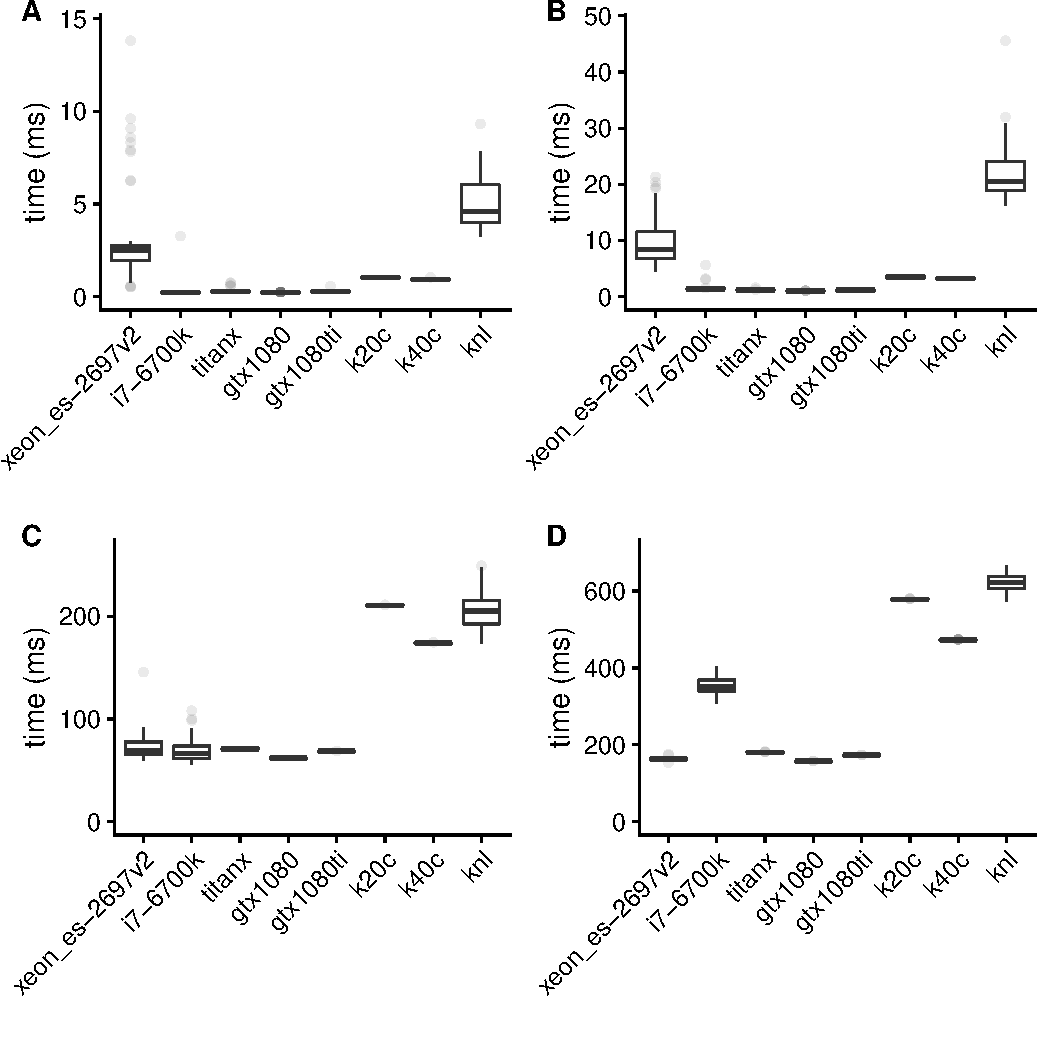
\includegraphics[width=1\textwidth]{figures/time-results/kmeans.pdf}
\caption{Kernel Execution times of the K-Means application over 4 different sized workloads, {\bf A} corresponds to {\bf tiny}, {\bf B} corresponds to {\bf small}, {\bf C} to {\bf medium} and {\bf D} to {\bf large}.}
\label{fig:time-kmeans}
\end{minipage}
\hfill
\begin{minipage}[b]{.45\textwidth}
\centering
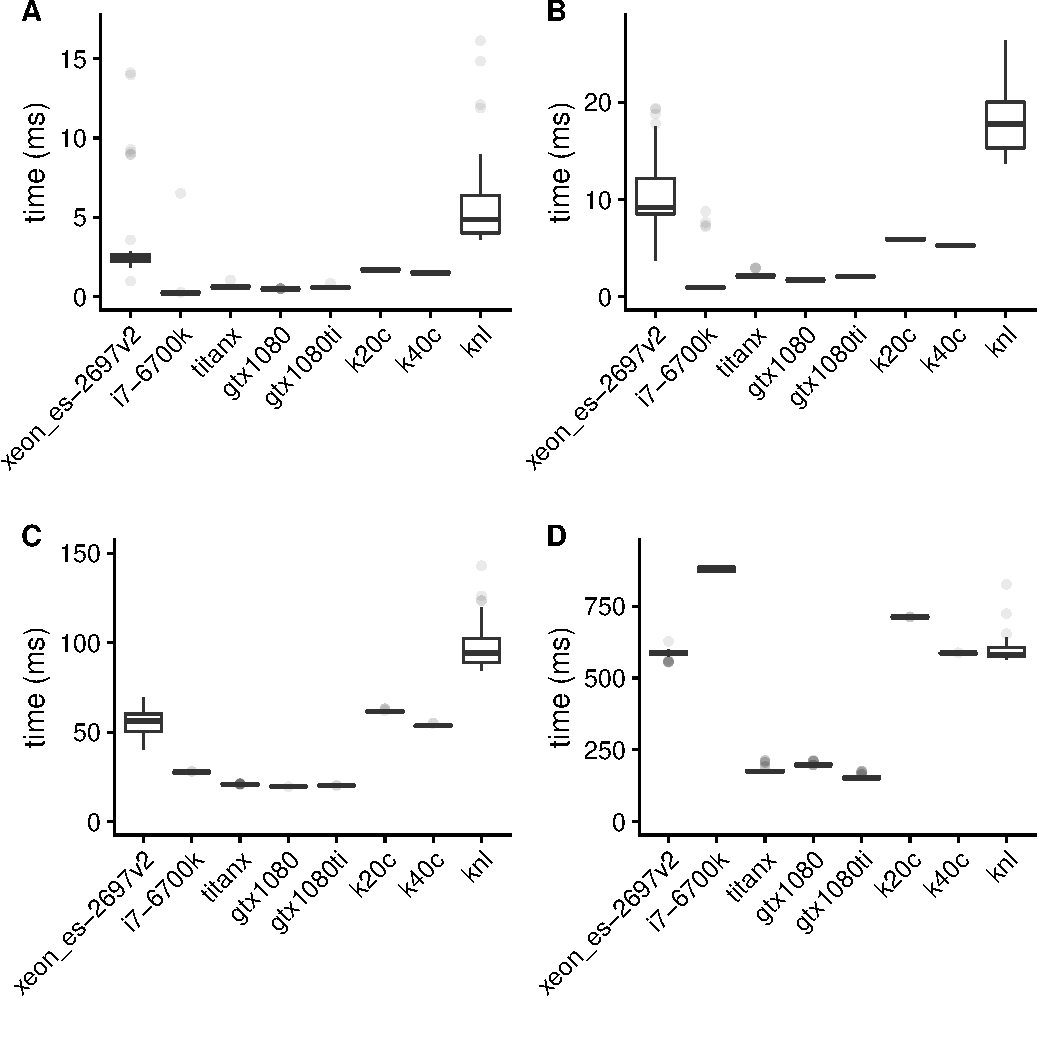
\includegraphics[width=1\textwidth]{figures/time-results/lud.pdf}
\caption{Kernel execution times over the LU-Decomposition application.}
\label{fig:time-lud}
\end{minipage}
\end{figure}

Sample execution times from running 50 iterations per benchmark application
\ref{fig:time-kmeans} \ref{fig:time-lud}

\end{document}
